% Options for packages loaded elsewhere
\PassOptionsToPackage{unicode}{hyperref}
\PassOptionsToPackage{hyphens}{url}
\PassOptionsToPackage{dvipsnames,svgnames,x11names}{xcolor}
%
\documentclass[
  12pt,
]{article}

\usepackage{amsmath,amssymb}
\usepackage{iftex}
\ifPDFTeX
  \usepackage[T1]{fontenc}
  \usepackage[utf8]{inputenc}
  \usepackage{textcomp} % provide euro and other symbols
\else % if luatex or xetex
  \usepackage{unicode-math}
  \defaultfontfeatures{Scale=MatchLowercase}
  \defaultfontfeatures[\rmfamily]{Ligatures=TeX,Scale=1}
\fi
\usepackage{lmodern}
\ifPDFTeX\else  
    % xetex/luatex font selection
  \setmainfont[]{Times New Roman}
\fi
% Use upquote if available, for straight quotes in verbatim environments
\IfFileExists{upquote.sty}{\usepackage{upquote}}{}
\IfFileExists{microtype.sty}{% use microtype if available
  \usepackage[]{microtype}
  \UseMicrotypeSet[protrusion]{basicmath} % disable protrusion for tt fonts
}{}
\makeatletter
\@ifundefined{KOMAClassName}{% if non-KOMA class
  \IfFileExists{parskip.sty}{%
    \usepackage{parskip}
  }{% else
    \setlength{\parindent}{0pt}
    \setlength{\parskip}{6pt plus 2pt minus 1pt}}
}{% if KOMA class
  \KOMAoptions{parskip=half}}
\makeatother
\usepackage{xcolor}
\usepackage[margin=1in]{geometry}
\setlength{\emergencystretch}{3em} % prevent overfull lines
\setcounter{secnumdepth}{-\maxdimen} % remove section numbering


\providecommand{\tightlist}{%
  \setlength{\itemsep}{0pt}\setlength{\parskip}{0pt}}\usepackage{longtable,booktabs,array}
\usepackage{calc} % for calculating minipage widths
% Correct order of tables after \paragraph or \subparagraph
\usepackage{etoolbox}
\makeatletter
\patchcmd\longtable{\par}{\if@noskipsec\mbox{}\fi\par}{}{}
\makeatother
% Allow footnotes in longtable head/foot
\IfFileExists{footnotehyper.sty}{\usepackage{footnotehyper}}{\usepackage{footnote}}
\makesavenoteenv{longtable}
\usepackage{graphicx}
\makeatletter
\def\maxwidth{\ifdim\Gin@nat@width>\linewidth\linewidth\else\Gin@nat@width\fi}
\def\maxheight{\ifdim\Gin@nat@height>\textheight\textheight\else\Gin@nat@height\fi}
\makeatother
% Scale images if necessary, so that they will not overflow the page
% margins by default, and it is still possible to overwrite the defaults
% using explicit options in \includegraphics[width, height, ...]{}
\setkeys{Gin}{width=\maxwidth,height=\maxheight,keepaspectratio}
% Set default figure placement to htbp
\makeatletter
\def\fps@figure{htbp}
\makeatother

\usepackage{amsmath}
\usepackage{amsfonts}
\usepackage{amssymb}
\usepackage{graphicx}
\usepackage{xcolor}
\usepackage{bm}
\usepackage{secdot}
\usepackage{mathptmx}
\usepackage{float}
\usepackage[utf8]{inputenc}
\usepackage{textcomp}
\usepackage[hang,flushmargin,bottom]{footmisc}
\usepackage{titlesec} \titleformat{\section}{\normalsize\bfseries}{\thesection.}{1em}{} \titleformat*{\subsection}{\normalsize\bfseries}
\usepackage{tocloft}
\usepackage{enumitem}
\usepackage[numbers,sort&compress]{natbib} \renewcommand{\bibsection}{} \setlength{\bibsep}{0.0pt}
\usepackage[hidelinks]{hyperref} \hypersetup{ colorlinks = true, urlcolor ={blue}, citecolor = {.}, linkcolor = {.}, anchorcolor = {.}, filecolor = {.}, menucolor = {.}, runcolor = {.} pdftitle={}, pdfsubject={}, pdfauthor={}, pdfkeywords={} } \urlstyle{same}
\usepackage{epstopdf}
\usepackage{fancyhdr, lastpage} \setlength{\topmargin}{-0.5in} \setlength{\headheight}{39pt} \setlength{\oddsidemargin}{0.25in} \setlength{\evensidemargin}{0.25in} \setlength{\textwidth}{6.0in} \setlength{\textheight}{8.5in}
\usepackage{caption} \captionsetup{font=small,labelfont=bf,figurename=Fig.,labelsep=period,justification=raggedright}
\makeatletter
\@ifpackageloaded{caption}{}{\usepackage{caption}}
\AtBeginDocument{%
\ifdefined\contentsname
  \renewcommand*\contentsname{Table of contents}
\else
  \newcommand\contentsname{Table of contents}
\fi
\ifdefined\listfigurename
  \renewcommand*\listfigurename{List of Figures}
\else
  \newcommand\listfigurename{List of Figures}
\fi
\ifdefined\listtablename
  \renewcommand*\listtablename{List of Tables}
\else
  \newcommand\listtablename{List of Tables}
\fi
\ifdefined\figurename
  \renewcommand*\figurename{Figure}
\else
  \newcommand\figurename{Figure}
\fi
\ifdefined\tablename
  \renewcommand*\tablename{Table}
\else
  \newcommand\tablename{Table}
\fi
}
\@ifpackageloaded{float}{}{\usepackage{float}}
\floatstyle{ruled}
\@ifundefined{c@chapter}{\newfloat{codelisting}{h}{lop}}{\newfloat{codelisting}{h}{lop}[chapter]}
\floatname{codelisting}{Listing}
\newcommand*\listoflistings{\listof{codelisting}{List of Listings}}
\makeatother
\makeatletter
\makeatother
\makeatletter
\@ifpackageloaded{caption}{}{\usepackage{caption}}
\@ifpackageloaded{subcaption}{}{\usepackage{subcaption}}
\makeatother
\ifLuaTeX
  \usepackage{selnolig}  % disable illegal ligatures
\fi
\usepackage{bookmark}

\IfFileExists{xurl.sty}{\usepackage{xurl}}{} % add URL line breaks if available
\urlstyle{same} % disable monospaced font for URLs
\hypersetup{
  pdftitle={Aligning Timescales and Frequency Combs},
  pdfauthor={Suzanne Thornton; Caitlin Berry; Amanda Koepke},
  colorlinks=true,
  linkcolor={blue},
  filecolor={Maroon},
  citecolor={Blue},
  urlcolor={Blue},
  pdfcreator={LaTeX via pandoc}}

\title{Aligning Timescales and Frequency Combs}
\author{Suzanne Thornton \and Caitlin Berry \and Amanda Koepke}
\date{2025-01-01}

\begin{document}
\maketitle

\newcommand{\pubnumber}{XXXX}
\newcommand{\DOI}{https://doi.org/10.6028/NIST.TN.XXXX}
\newcommand{\monthyear}{Month Year}

\urlstyle{rm}

\begin{titlepage}
    \begin{flushright}
 
\LARGE{\textbf{NIST Technical Note XXXX}}\\
\vfill
 
\Huge{\textbf{Aligning Timescales and Frequency Combs}}\\
\vfill
 
\large Suzanne Thornton\\
\large Caitlin Berry\\
\large Amanda Koepke\\
\vfill
 
\normalsize This publication is available free of charge from:\\
https://doi.org/10.6028/NIST.TN.XXXX\\
\vfill
 


\includegraphics[width=0.3\linewidth]{NIST-logo.eps}\\ 


\end{flushright}
\end{titlepage}
\begin{titlepage}
 
\begin{flushright}
 
\LARGE{\textbf{NIST Technical Note XXXX}}\\
\vfill 
 
\Huge{\textbf{Title}}\\
\vfill
 
\normalsize First Author\\
Second Author\\
\textit{Office of XXXX}\\
\textit{First Operating Unit}\\
\vspace{12pt}
Third Author\\
Fourth Author\\
\textit{Office of XXXX}\\
\textit{Second Operating Unit}\\
\vfill
 
\normalsize This publication is available free of charge from:\\
https://doi.org/10.6028/NIST.TN.XXXX\\
\vfill
 
\normalsize Month Year
\vfill
    


\includegraphics[width=0.18\linewidth]{DoC-logo.eps}\\ 
\vfill
 
\footnotesize U.S. Department of Commerce\\ 
\textit{Gina M. Raimondo, Secretary}\\
\vspace{10pt}
National Institute of Standards and Technology\\ 
\hspace*{-3cm}\textit{James K. Olthoff, Performing the Non-Exclusive Functions and Duties of the Under Secretary of Commerce \\
for Standards and Technology \& Director, National Institute of Standards and Technology} 
\end{flushright}
\end{titlepage}

\begin{titlepage}
 
\begin{flushright}
\footnotesize  Certain commercial entities, equipment, or materials may be identified in this document in order to describe an experimental procedure or concept adequately. Such identification is not intended to imply recommendation or endorsement by the National Institute of Standards and Technology, nor is it intended to imply that the entities, materials, or equipment are necessarily the best available for the purpose.\\ 
\vfill
 
\normalsize \textbf{National Institute of Standards and Technology Technical Note XXXX\\ 
Natl. Inst. Stand. Technol. Tech. Note XXXX, \pageref{LastPage} pages (Month Year)} \\
\textbf{CODEN: NTNOEF}\\
\vspace{12pt}
\textbf{This publication is available free of charge from: https://doi.org/10.6028/NIST.TN.XXXX}
\vfill
\end{flushright}
\end{titlepage}

\section*{Abstract}

\normalsize Required

\section*{Key words}

\normalsize Required, alphabetized, separated by semicolon, and end in a
period. \pagebreak

\begin{center}
    \tableofcontents
    \listoftables
    \listoffigures
\end{center}
\pagebreak

\section*{Glossary}

Delete if not applicable \pagebreak

\section{Introduction}

\subsection{All Subsection Headings Capitalized}\label{subsec:headingscap}

This can be seen in Eq. (1) and Table 1. Information about flowers is
available in Sec.\ref{sec:intro} .\footnote{NIST disclaimer text here.}

\begin{equation}
{x}^{n} + {y}^{n} = {z}^{n}
\end{equation}

\begin{itemize}
\item Initial input: Independent series of clock and comb data
\begin{itemize}
    \item Clock shift files containing variables: MJD, shift, and possibly ISGOOD 
    \item Frequency comb data containing variables: MJD, SDR:frep ErYb, fo ErYb, fb Si ErYb, fb Al ErYb, fb Yb ErYb
\end{itemize}
\item Read data into Python
\item Define functions to find optical frequencies for each clock with comb equation, these frequencies will become additional variables in the frequency comb data object 
\item compute total correction for each clock's shift data 
\item Data processing 
\begin{itemize}
    \item change all data variables to type float for high precision computing
    \item find overlapping MJD values for each clock frequency data set 
    \item visualize gaps in the clock frequency data sets 
    \item decide upon initial and final MJD values for analysis  
\end{itemize} 
\item Imputation -  decide how to deal with missing shift values
\begin{itemize}
    \item adjust start/end MJD indices for large gaps of missing values 
    \item use interpolation techniques (see below) for short sequence of individual missing values 
    \item keep with caution about how this may impact subsequent steps 
\end{itemize}
\item Interpolation - to get clock data to match up with comb time intervals, key difference from imputation step is data is contained w/in a certain range of start/stop MJD values 
\begin{itemize}
    \item numpy.interp, linear 
    \item pandas.interpolate, linear 
    \item incorporate randomness 
    \item kalman smoothing 
\end{itemize}
\item Calculate clock frequencies by adding together comb frequencies and shift data, scaled by the total correction amount 
\item End results: clock ratio data to compute offset to compare to previous measurements (may contain missing values?) 
\end{itemize}

\begin{table}[H]
    \centering
    \caption{Title.}
    \small
    \begin{tabular}{cc}
        \hline
        ColumnA & ColumnB \\ \hline
        text & text{\scriptsize $^{\textrm a}$} \\
        text & text \\
        text & text \\
        text & text \\
        \hline
    \end{tabular}
    
    {\footnotesize  {\scriptsize $^{\textrm a}$}Footnote}
\end{table}

\begin{figure}[h] 
    \centering  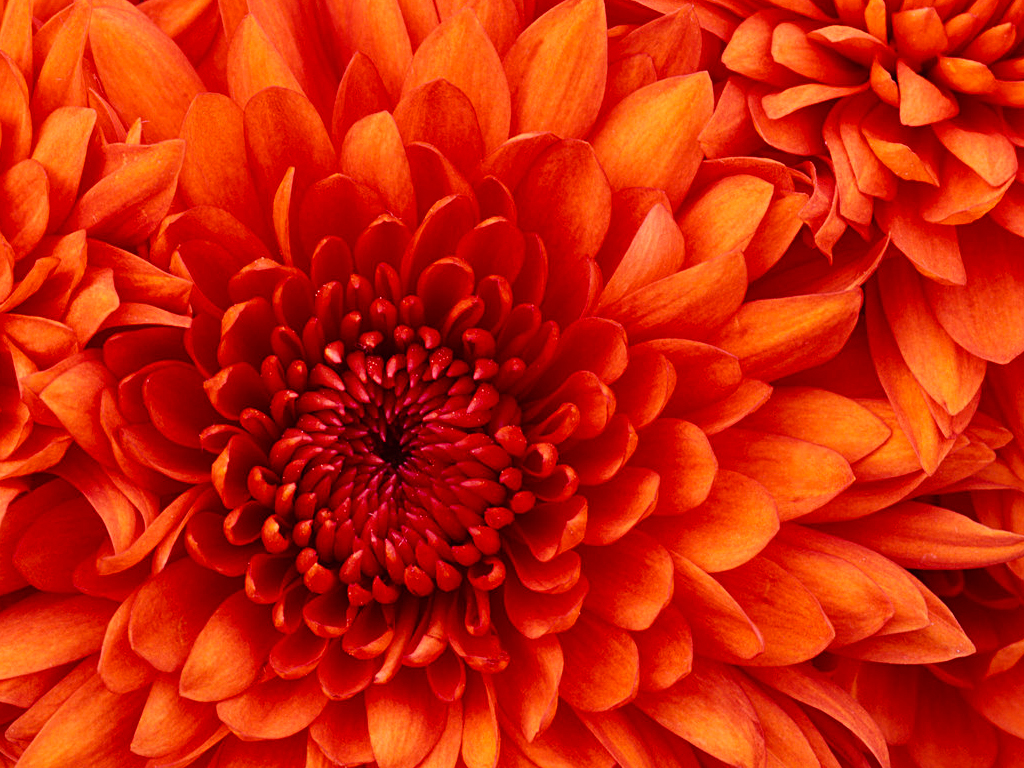
\includegraphics[width=0.5\linewidth]{Chrysanthemum.jpg}
    \caption{This is the caption text.}
    \label{fig:Chrysanthemum}
\end{figure}



\end{document}
